\section{Слой представления}
	В качестве фреймворка для слоя представления была выбрана технология Spring MVC. Данная технология позволяет реализовать паттерн Model-View-Controller при помощи слабо связанных компонентов. В качестве модели выступает слой бизнес-логики приложения. Контроллеры реализованы в виде RESTful контроллеров с помощью фреймворка Spring. Представление реализовано с помощью JavaScript фреймворка AngularJS и HTML страниц. Работа происходит по следующему сценарию:
	\begin{enumerate}
		\item RESTful сервис принимает запрос от пользователя;
		\item сервис вызывает соответствующие методы бизнес логики для обработки запроса;
		\item сервис возвращает ответ на запрос в виде JSON-объекта;
		\item AngularJS клиент получает ответ от сервера и рэндерит соответствующую HTML-страницу и показывает его в браузере.
	\end{enumerate}
	
	Рассмотрим более подробно REST API, предоставляемый сервером.
	\begin{itemize}
		\item \texttt{UserController}
		\begin{itemize}
			\item URL: \texttt{"rest/user/:login"} --- получение пользователя с логином \texttt{login}
			\item URL: \texttt{"rest/user/:login"}, метод POST --- регистрация нового пользователя
			\item URL: \texttt{"rest/user/:login/authenticate"} --- аутентификация пользователя
			\item URL: \texttt{"rest/user/:login/messages"} --- получить все уведомления для пользователя
			\item URL: \texttt{"rest/user/:login/projects"} --- получить все проекты, в которых участвует пользователя
			\item URL: \texttt{"rest/user/:login/projects"}, метод POST --- добавление нового проекта пользователю
			\item URL: \texttt{"rest/user/:login/managed\_tickets"} --- получить все тикеты, которыми руководит пользователь
			\item URL: \texttt{"rest/user/:login/assigned\_tickets"} --- получить все тикеты, которые разрабатывает пользователь
			\item URL: \texttt{"rest/user/:login/managed\_reports"} --- получить все ошибки, которыми руководит пользователь
			\item URL: \texttt{"rest/user/:login/assigned\_reports"} --- получить все ошибки, которые разрабатывает пользователь
		\end{itemize}
		
		\item \texttt{TicketController}
		\begin{itemize}
			\item URL: \texttt{"rest/ticket/:id"} --- получение тикета с идентификатором \texttt{id}
			\item URL: \texttt{"rest/ticket/:id/permissions"} --- получение прав пользователя для тикета
			\item URL: \texttt{"rest/ticket/:id/milestone"} --- получение майлстоуна тикета
			\item URL: \texttt{"rest/ticket/:id"}, метод PUT --- установить новый статус тикету
			\item URL: \texttt{"rest/ticket/:id/assignees"} --- получить всех разработчиков тикета
			\item URL: \texttt{"rest/ticket/:id/assignees"}, метод POST --- добавить нового разработчика в тикет
			\item URL: \texttt{"rest/ticket/:id/comments"} --- получить все комментарии тикета
			\item URL: \texttt{"rest/ticket/:id/comments"}, метод POST --- добавить новый комментарий тикету
		\end{itemize}
		
		\item \texttt{ReportController}
		\begin{itemize}
			\item URL: \texttt{"rest/report/:id"} --- получение отчета с идентификатором \texttt{id}
			\item URL: \texttt{"rest/report/:id/permissions"} --- получение прав пользователя для отчета
			\item URL: \texttt{"rest/report/:id/project"} --- получение проекта отчета
			\item URL: \texttt{"rest/report/:id"}, метод PUT --- установить новый статус отчету
			\item URL: \texttt{"rest/report/:id/comments"} --- получить все комментарии отчета
			\item URL: \texttt{"rest/report/:id/comments"}, метод POST --- добавить новый комментарий отчету
		\end{itemize}
		
		\item \texttt{ProjectController}
		\begin{itemize}
			\item URL: \texttt{"rest/project/:name"} --- получение проекта с именем \texttt{name}
			\item URL: \texttt{"rest/project/:name"}, метод PUT --- обновить проект с именем \texttt{name}
			\item URL: \texttt{"rest/project/:name/permissions"} --- получение прав для проекта
			\item URL: \texttt{"rest/project/:name/reports"} --- получение ошибок для проекта
			\item URL: \texttt{"rest/project/:name/reports"}, метод POST --- добавление ошибки в проект
			\item URL: \texttt{"rest/project/:name/milestones"} --- получение майлстоунов для проекта
			\item URL: \texttt{"rest/project/:name/milestones"}, метод POST --- добавление майлстоуна в проект
			\item URL: \texttt{"rest/project/:name/developers"} --- получение разработчиков проекта
			\item URL: \texttt{"rest/project/:name/developers"}, метод POST --- добавление разработчика в проект
			\item URL: \texttt{"rest/project/:name/testers"} --- получение тестировщиков проекта
			\item URL: \texttt{"rest/project/:name/testers"}, метод POST --- добавление тестировщика в проект
		\end{itemize}
		
		\item \texttt{MilestoneController}
		\begin{itemize}
			\item URL: \texttt{"rest/milestone/:id"} --- получение майлстоуна с идентификатором \texttt{id}
			\item URL: \texttt{"rest/milestone/:id/permissions"} --- получение прав пользователя для майлстоуна
			\item URL: \texttt{"rest/milestone/:id/project"} --- получение проекта майлстоуна
			\item URL: \texttt{"rest/milestone/:id"}, метод PUT --- установить новый статус майлстоуну
			\item URL: \texttt{"rest/milestone/:id/tickets"} --- получить все тикеты майлстоуна
			\item URL: \texttt{"rest/milestone/:id/tickets"}, метод POST --- добавить новый тикеты майлстоуну
		\end{itemize}	
	\end{itemize}
	
	При возникновении неполадок на стороне сервера, выбрасывается соответствующее исключение. Данное исключение перехватывается с помощью специальных инструментов и генерируется HTTP ответ, который содержит код и сообщение с описанием ошибки.
	
	Клиентская сторона посылает запросы к соответствующим RESTful сервисам и затем рэндерит соответствующую HTML страницу. Работа с REST API происходит с помощью библиотеки Angular Resource. Пример angular-контроллера приведен на листинге
	\begin{lstlisting}[style=crs_js, label={lst:jsController}, caption={Angular-контроллер}]
	/**
	* Created by kivi on 18.12.17.
	*/
	
	function ReportService($resource) {
	return $resource('rest/report/:id', {id: '@id'});
	}
	
	function ReportPermService($resource) {
	return $resource('rest/report/:id/permissions?user=:login', {id: '@id', login: '@login'});
	}
	
	function ReportProjectService($resource) {
	return $resource('rest/report/:id/project', {id: '@id'});
	}
	
	function ReportCommentService($resource) {
	return $resource('rest/report/:id/comments?user=:login', {id: '@id', login: '@login'});
	}
	
	function ReportController($scope, $http, $routeParams,
	ReportService,
	ReportPermService,
	ReportCommentService,
	ReportProjectService,
	InfoShareService) {
	function url() {
	return {id: $routeParams.id};
	}
	function url_with_login(login) {
	return {id: $routeParams.id, login:login};
	}
	
	this.user = InfoShareService.getUser();
	this.permissions = ReportPermService.get(url_with_login(this.user.login));
	this.project = ReportProjectService.get(url());
	this.instance = ReportService.get(url());
	this.comments = ReportCommentService.query(url());
	
	this.changeStatus = function (status) {
	$http.put('rest/report/' + this.instance.id + '?user=' + this.user.login, status)
	.then(function () {
	this.update();
	}.bind(this), function (error) {
	alert(error.data.message);
	});
	};
	
	this.commentReport = function () {
	if (isEmpty($scope.reportComment)) {
	alert("Enter comment message");
	} else {
	var comment = new ReportCommentService();
	comment.description = $scope.reportComment;
	comment.$save(url_with_login(this.user.login), function () {
	$scope.reportComment = "";
	this.updateComments();
	}.bind(this), function (error) {
	alert(error.data.message);
	});
	}
	};
	
	this.update = function () {
	this.instance = ReportService.get(url());
	};
	
	this.updateComments = function () {
	this.comments = ReportCommentService.query(url());
	}
	}
	
	app
	.factory('ReportService', ReportService)
	.factory('ReportPermService', ReportPermService)
	.factory('ReportProjectService', ReportProjectService)
	.factory('ReportCommentService', ReportCommentService)
	.controller('ReportController', ReportController);
	\end{lstlisting}
	
	Скриншоты пользовательского интерфейса приведены на рисунках~\ref{fig:loginPage} -- \ref{fig:reportPage}.
	
	\begin{figure}[h]
		\center{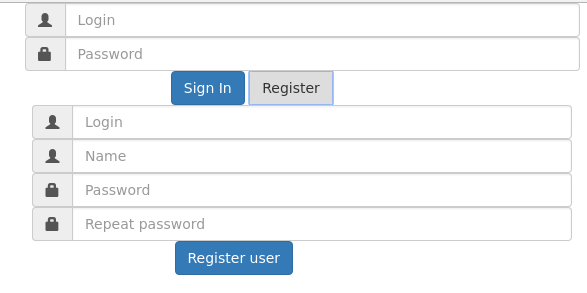
\includegraphics[width=\linewidth]{loginPage}}
		\caption{Страница входа}
		\label{fig:loginPage}
	\end{figure}
	\begin{figure}[h]
		\center{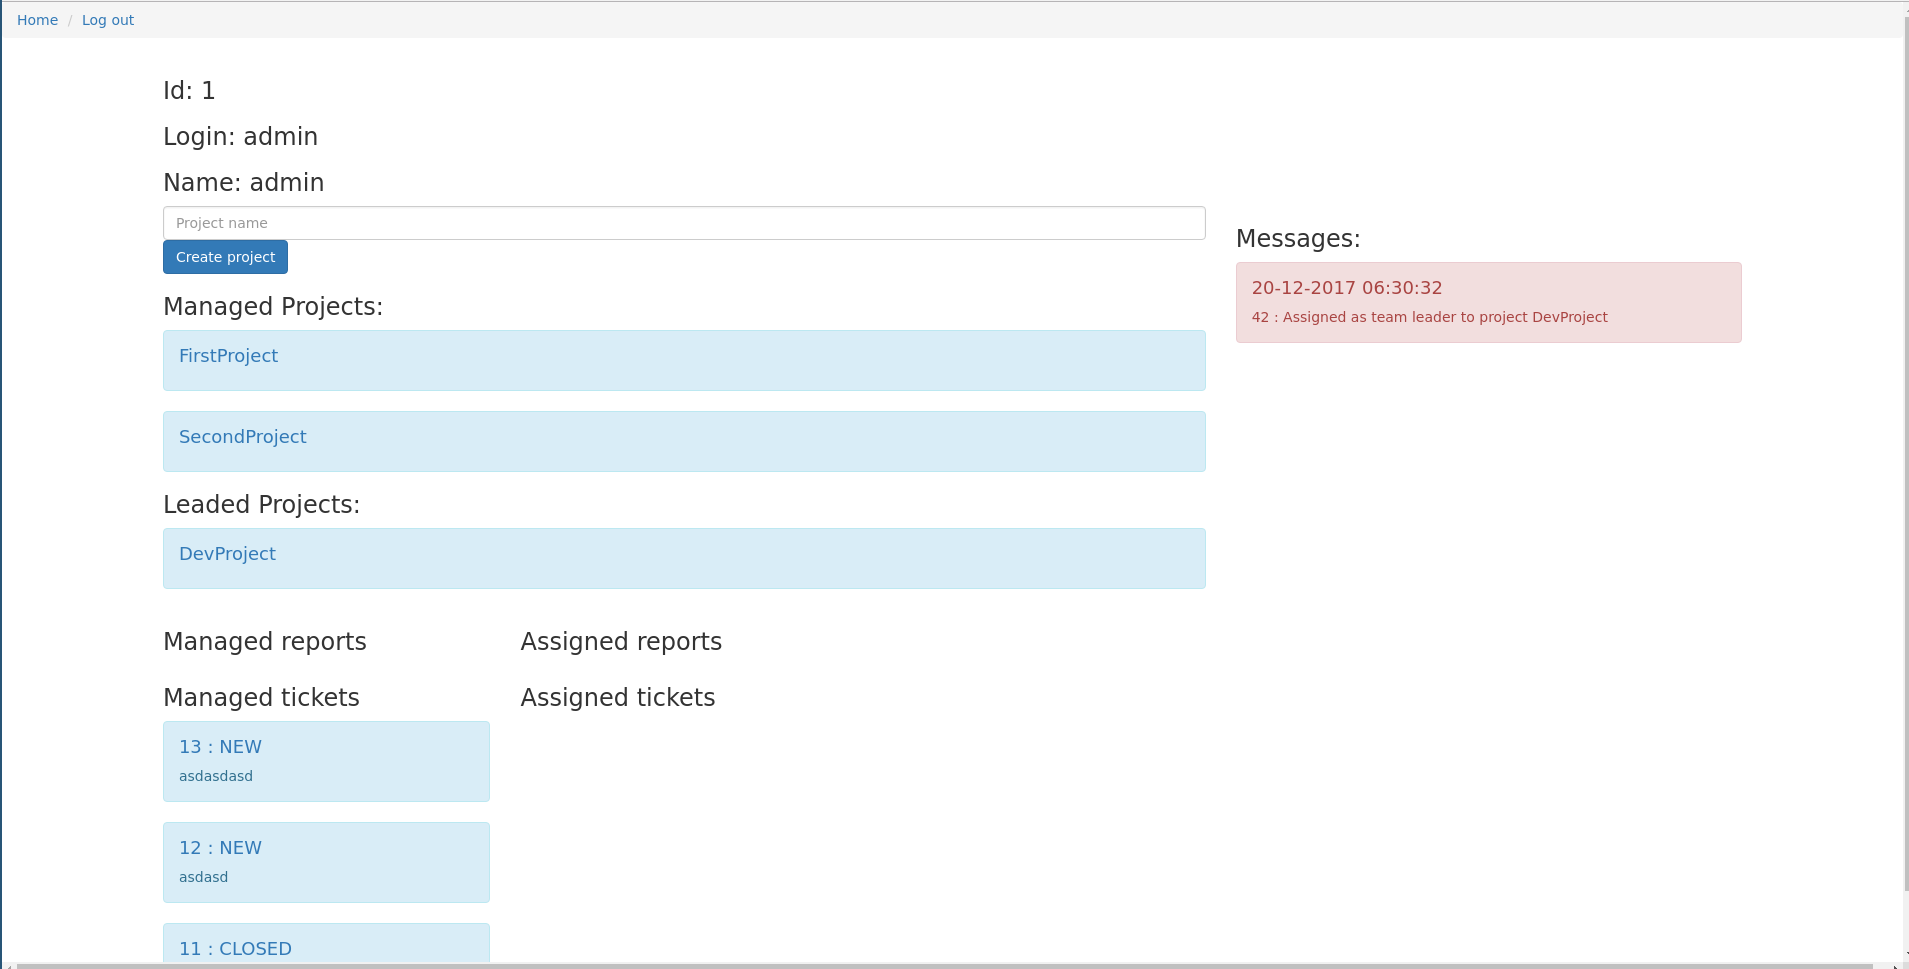
\includegraphics[width=\linewidth]{userPage}}
		\caption{Страница пользователя}
		\label{fig:userPage}
	\end{figure}
	\begin{figure}[h]
		\center{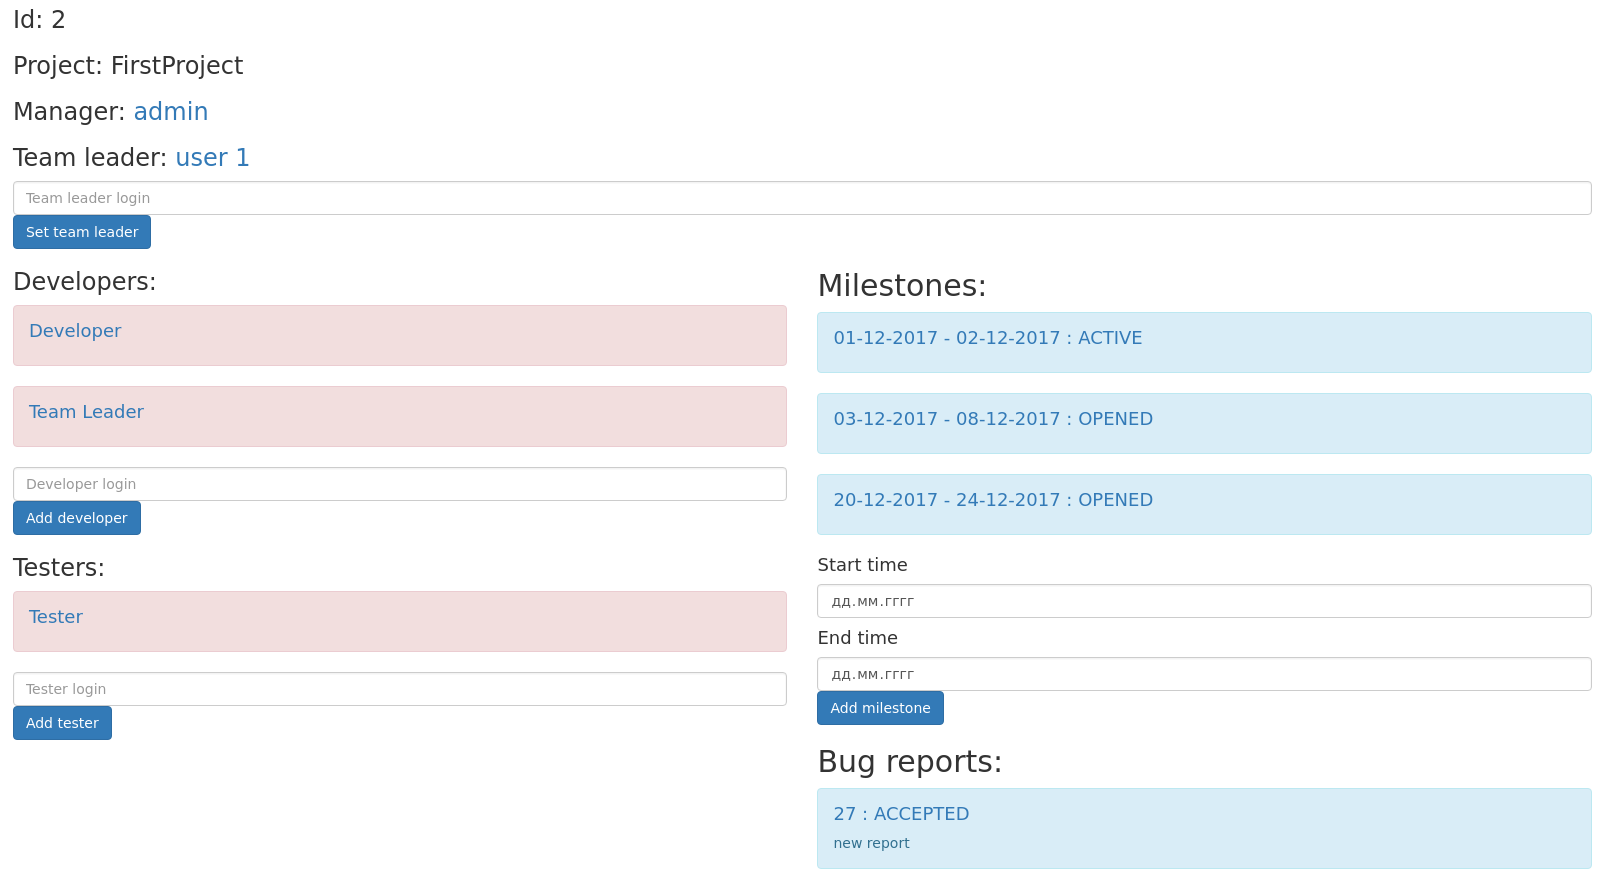
\includegraphics[width=\linewidth]{projectPage}}
		\caption{Страница проекта}
		\label{fig:projectPage}
	\end{figure}
	\begin{figure}[h]
		\center{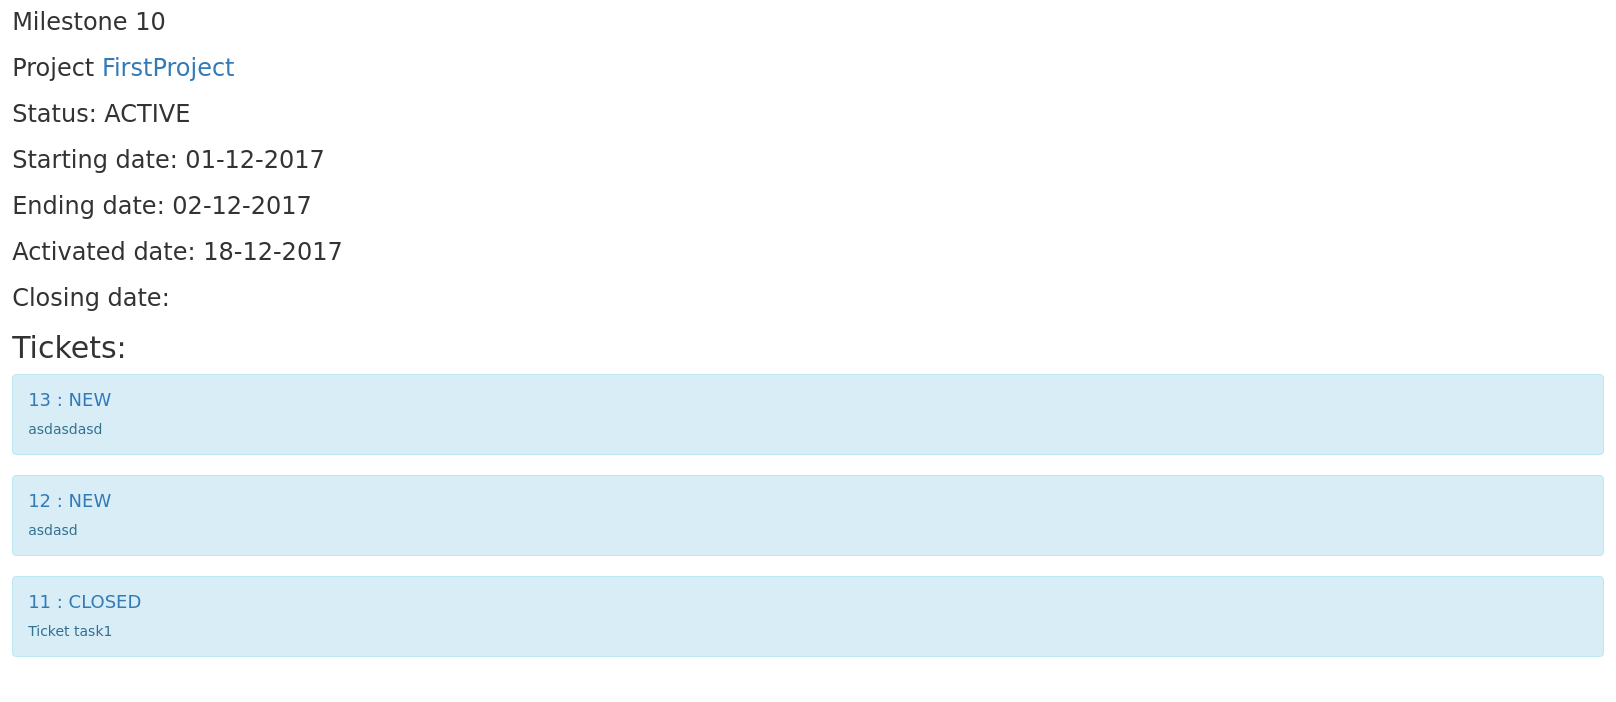
\includegraphics[width=\linewidth]{milestonePage}}
		\caption{Страница майлстоуна}
		\label{fig:milestonePage}
	\end{figure}
	\begin{figure}[h]
		\center{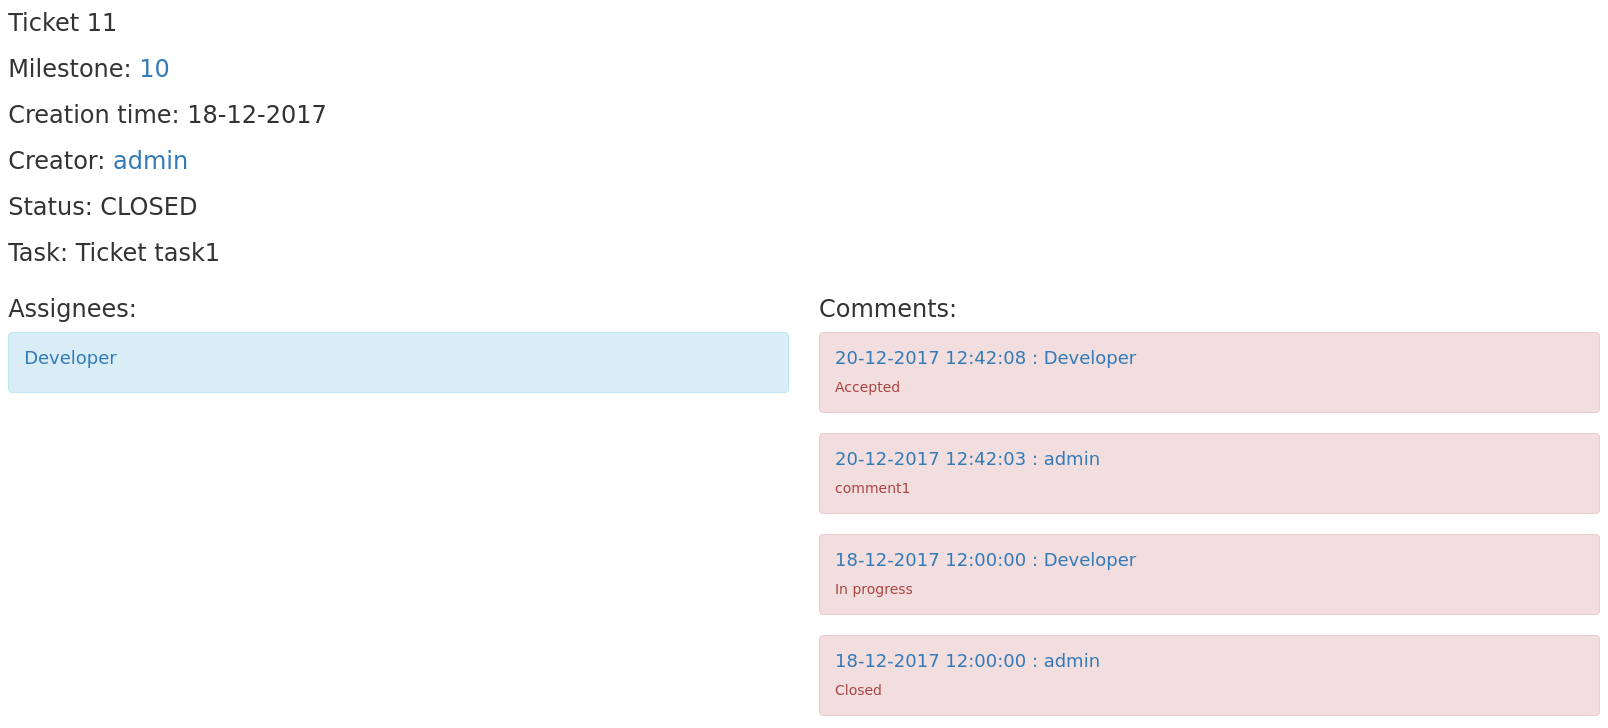
\includegraphics[width=\linewidth]{ticketPage}}
		\caption{Страница тикета}
		\label{fig:ticketPage}
	\end{figure}
	\begin{figure}[h]
		\center{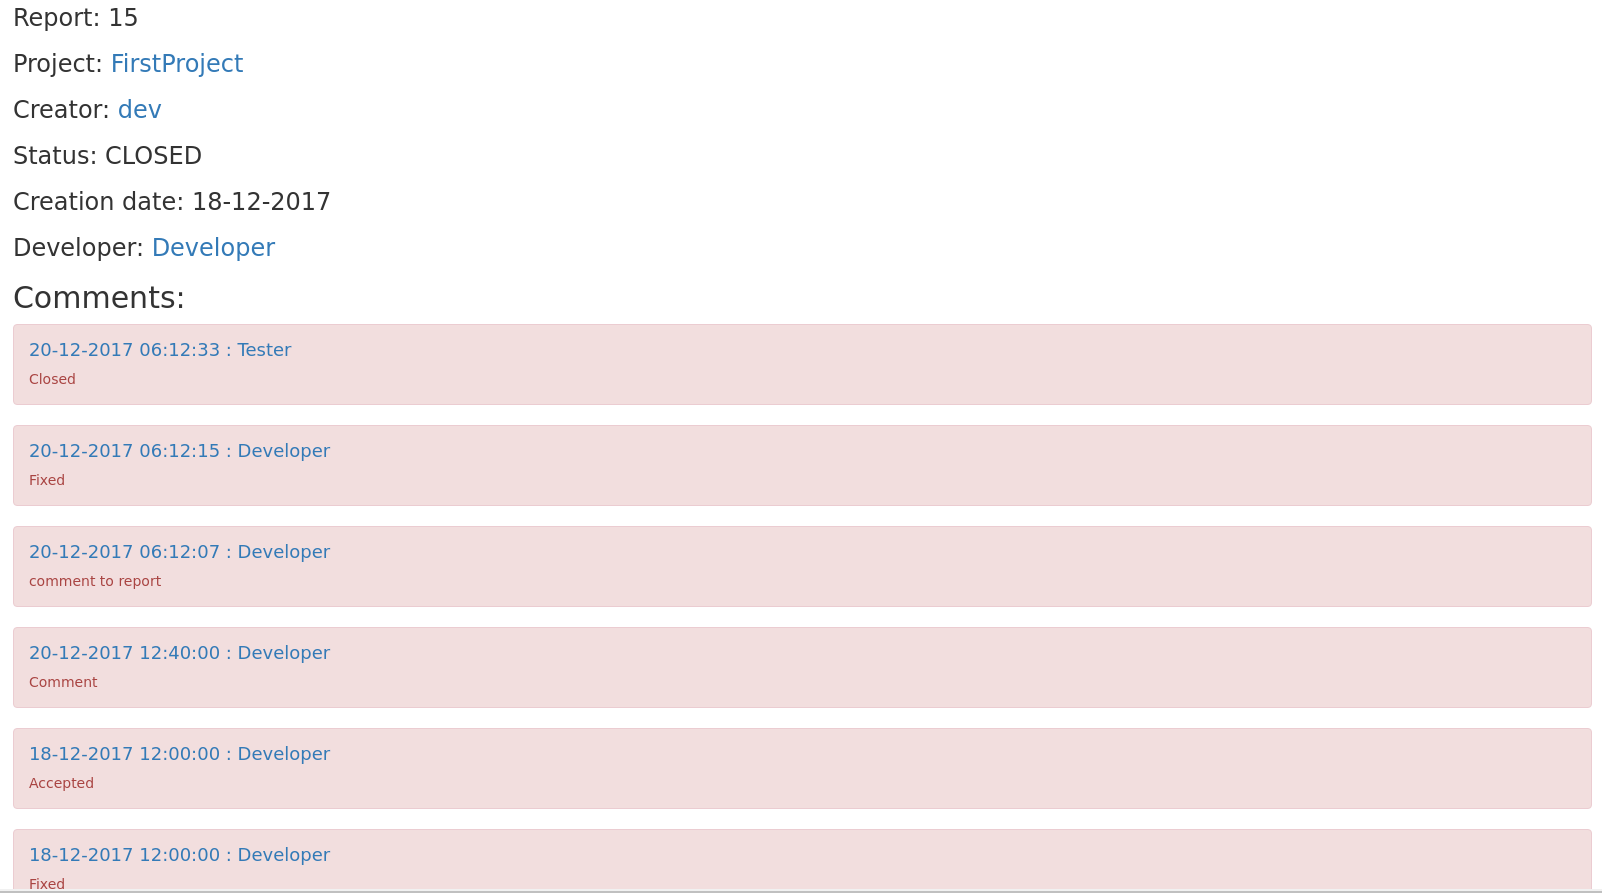
\includegraphics[width=\linewidth]{reportPage}}
		\caption{Страница отчета об ошибке}
		\label{fig:reportPage}
	\end{figure}